\chapter{Characteristic of wood}
\label{Chapter1}

\section{introduction}

In this section, the mechanical properties of wood are reminded. Wood is a heterogeneous material and sensitive to moisture. Indeed, the humidity of wood is an important characteristic that has consequences on its physical and mechanical properties. Moisture content and temperature are two parameters that will greatly influence the behavior of wood material. The variation of humidity will lead to variations of dimensions, shape, volume, density and thus resistance of the wood. 

Trees are one of the most important living reservoirs of carbon monoxide. Through the phenomenon called photosynthesis, they absorb carbon dioxide and release oxygen into the atmosphere. Wood is used for many applications. It can be used as energy, in timber frames and constructions, for packaging, in furniture and carpentry, in the paper industry or in the chemical industry for example. This document is based on the study of a resinous wood; the pine specimen which presents a less complex structure than the hardwoods. In this part, the material wood will be presented with its physical aspects and its mechanical properties. The macroscopic and microscopic aspects will be also reminded.

\section{Generalities}

\subsection{The wood}

Wood is defined as 'a set of very resistant tissues that constitute the trunk, branches and roots of woody plants, formed by vessels conducting raw sap, fibres and parenchyma' (figure 1). In other words, wood is a set of tissues composed of woody fibres, tracheids parenchyma and vessels.

\graphicspath{{Images/}}
\begin{figure}[htp]
	\centering
	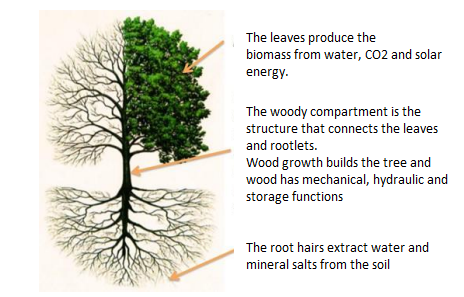
\includegraphics[width=8cm]{fig1}
	\caption{The main functions of the tree's wood[THI 2015]}
	\label{fig:galaxy}
\end{figure}

The wood ensures in trees 3 main functions: the conduction of the raw sap from the roots to the branches, the mechanical support of the whole tree against its own weight and external forces, and the storage of nutrients such as starch. It is one of the few $100 \%$ natural materials. Its main chemical components are carbon, oxygen and hydrogen. Its use allows to limit greenhouse gas emissions and thus to fight against global warming. The tree absorbs carbon with which it manufactures the cells of the wood and rejects oxygen in the atmosphere. Wood is a natural material, renewable, transformable at low energy cost, recyclable, biologically degradable. For construction, it has advantages and disadvantages presented in table 1:

\graphicspath{{Images/}}
\begin{figure}[htp]
	\centering
	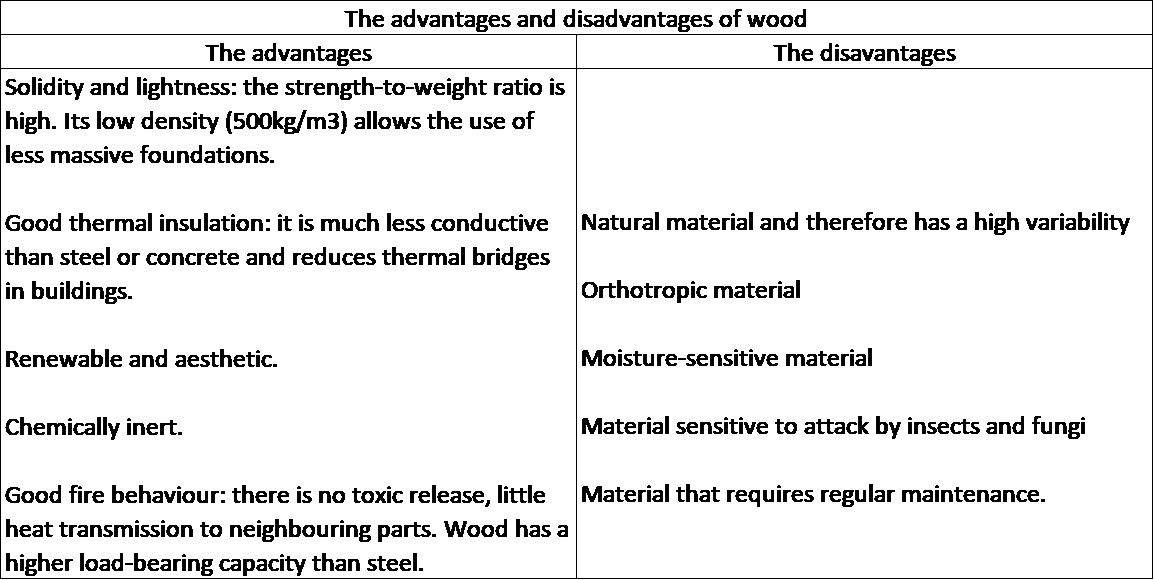
\includegraphics[width=12cm]{fig2}
	\caption{The advantages and disadvantages of wood}
	\label{fig:galaxy}
\end{figure}

\subsection{Two characteristics of the tree's wood}

Wood has two important characteristics which are anisotropy and heterogeneity. Anisotropy is a direct consequence of its heterogeneity.

\begin{itemize}
	\item It is heterogeneous by the fact that it is made up of various natures and forms that are the cells. 
	\item It is anisotropic because its elements are oriented in several directions. Its mechanical and physical properties are not the same in all planes. The material is also orthotropic which means it has 3 preferred directions: longitudinal, radial and tangential.
\end{itemize}

In order to facilitate the studies on the physical and mechanical behaviours, we take as reference three types of sections as shown in Figure 2 and defined as follows:

\begin{itemize}
	\item Cross-section (T), perpendicular to the shaft of the tree (trunk). When we look at a freshly felled tree, we can easily imagine a cross-section with the annual growth rings at the end, which correspond to the woody material produced by the tree in spring or summer.
	\item Tangential section (L), longitudinal, in the direction of the wood grain, and perpendicular to the medullary rays centered on the core of the log. During the cutting of the log into logs (current cutting), the patterns of the faces of the first boards obtained are characteristic.
	\item Radial section (R), again longitudinal, and in the direction of the wood grain, but parallel
	to the rays. This section can be seen on trays cut near the heart.
\end{itemize}

\graphicspath{{Images/}}
\begin{figure}[htp]
	\centering
	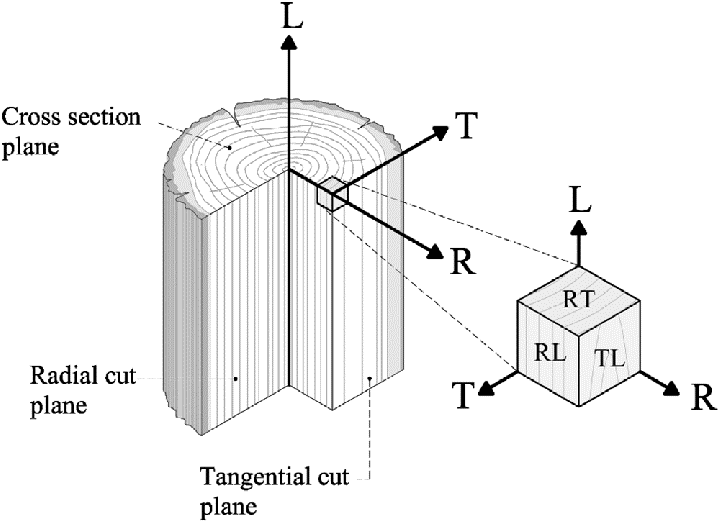
\includegraphics[width=10cm]{fig3}
	\caption{Main orthotropic directions and planes in Wood}
	\label{fig:galaxy}
\end{figure}

\section{Macroscopic and microscopic structure of wood}

\subsection{Macroscopic Scale}

The wood grows in concentric layers to the outside. It is this growth that creates heterogeneity [SED 2006]. Figure 3 shows the different elements that participate in the growth of a tree:

\graphicspath{{Images/}}
\begin{figure}[htp]
	\centering
	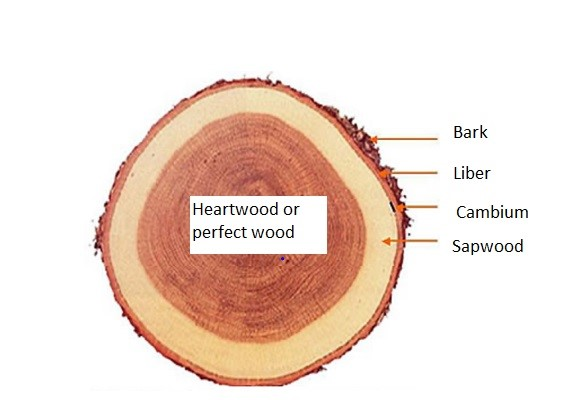
\includegraphics[width=8cm]{fig4}
	\caption{Sectional view of the wood}
	\label{fig:galaxy}
\end{figure}

\begin{itemize}
	\item Outer bark: consists of dead cells and serves to protect the tree. It surrounds the tree to protect the cambium and the deep layer from climatic, animal or physical attack. 
	\item Inner bark (Liber): A layer of cells in which the elaborated (descending) sap circulates
	\item Cambium: Produces the bast towards the outside and the wood (xylem) towards the inside (growth tissue). This part can develop into sapwood or the next layer, the bark. It is therefore a particular part that explains the growth of the tree's circumference.
	\item Sapwood: Incompletely completed wood in which the raw sap circulates. The sap allows water and nutrients to be transmitted from the soil to all parts of the tree.
	\item Heartwood or perfect wood (dead cells) is the wood with the best mechanical properties. It is considered to be the dead part of the wood which is darker in colour than the other parts. It is the most used part of the tree for construction.
	\item Pith (heart) central part consisting of spongy tissue
\end{itemize}

There is sometimes a difference in colour between sapwood and heartwood (in the case of differentiated woods: oak, chestnut, pine, Douglas fir, larch). Sapwood is not or only slightly resistant to damage, whereas heartwood, which is not very impregnable, is naturally resistant. Conversely, for non-differentiated woods (fir, spruce, poplar, maple), the two parts are not visually distinguishable. However, there are different porosity and therefore different absorption capacities.

\subsection{Microscopic Scale}

Microscopically, there are two types of wood made up of different types of plant tissue: softwoods and hardwoods. Figures 4 presents microscopically these two categories of wood.

Softwoods are older than hardwoods and therefore have a simpler structure. They are made up of two main groups of cells: tracheids and parenchyma cells. The observation of these two types of cells shows the following configuration:

\begin{itemize}
	\item Tracheid fibers, having both support and conduction roles
	\item Rays: tracheid fibers and horizontal parenchyma
	\item Vertical parenchyma which ensure the distribution and storage of substances.
\end{itemize}

Hardwoods have more cell diversity than softwoods. They are composed of different cells: vessels, tracheids and parenchyma. The functions of support and conduction are performed by different cells:

\begin{itemize}
	\item Fibers (librifomes and tracheids): they are bundles of resistant cells, arranged in the axial direction, they ensure the rigidity and the mechanical resistance of wood. It is a bio composite made of cellulose, hemicellulose and lignin;
	\item Vessels: these are hollow cells that serve to conduct the raw sap from the roots to the leaves;
	\item Vertical parenchyma: this consists of parenchymal cells that contribute to the transport of nutrients. These parenchyma, associated with the vessels, give particular patterns to each species on the cross section;
	\item Woody rays (or medullary rays): these are horizontal parenchyma made up of thickened and lignified reserve cells with thickened and lignified walls. They accompany the vascular tissue. These cells participate in the support function of the tree. Their orientation is transverse and radiating from the longitudinal axis of the shaft.
\end{itemize}

\graphicspath{{Images/}}
\begin{figure}[htp]
	\centering
	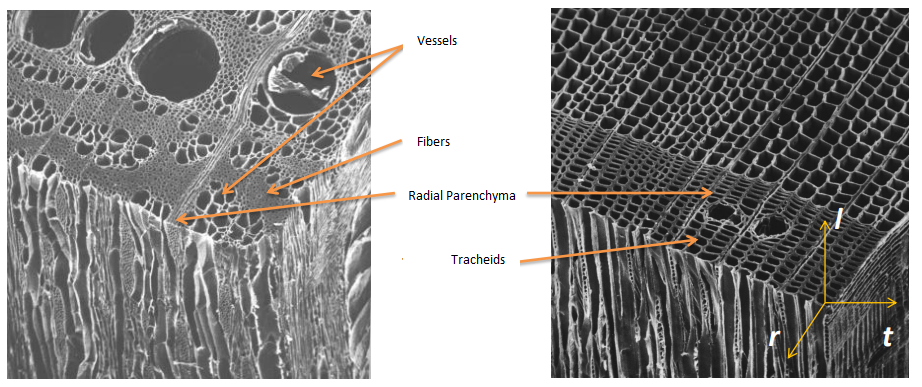
\includegraphics[width=10cm]{fig5}
	\caption{Microscopic section of hardwood and softwood [THI 2015]}
	\label{fig:galaxy}
\end{figure}

\subsection{Chemical composition of wood}

Wood is a set of tissues of more or less hard consistency forming the main mass of the trunk of trees. It is an organized and heterogeneous material formed by a set of fibers accumulated by trees during their progressive growth over successive years. The structure of the tree is made up of cells (dead or alive) that ensure the circulation of sap, the storage of nutritive reserves and defense against possible aggressions.
The elemental chemical composition of wood organic matter varies very little from one species to another. On average, wood is made up of $50 \%$ carbon, $42 \%$ oxygen, $6 \%$ hydrogen, $1 \%$ nitrogen and $1 \%$ minerals. Wood is essentially composed of 3 types of polymers: cellulose, hemicelluloses and lignins. There are other components called extractives that do not contribute to the mechanical properties of the wood, but rather play the role of protection against the attacks of insects and other parasites.

\smallskip

\textbf{Lignin}

Its quantity in the wood represents $20 \%$ to $30 \%$. Lignin is a molecule that is part of the different components of wood. We found in some algae and in plants that have roots. It is the element which brings to wood its rigidity, its impermeability and its strength against decomposition. Trees are the plants that contain the most lignin. The lignin molecules allow the plants to stand upright to access to the light.

\smallskip

\textbf{Hemicelluloses}

The proportion of hemicelluloses in wood is estimated between $15 \%$ and $25 \%$. These are amorphous and branched polymers made up of units of different sugar residues. The hemicelluloses play a bridging role between the cellulose fibers.

\smallskip

\textbf{Cellulose}

It is the dominant constituent of wood (about $50 \%$). It is the most abundant organic matter on earth. The role of the fibrils, dispersed in an amorphous matrix of celluloses of a plastic nature, is to transform the latter into an elastic system with a high tensile strength, especially if the fibrils are small in diameter: about 2 nm in the primary walls.

\section{Mechanical behaviour}

In this section the physical and mechanical properties of wood are presented. Different factors influence the properties of wood such as the type of species, growing conditions and moisture content. Wood is considered to be an anisotropic material, meaning that its properties vary in different directions.The orthotropy, viscosity and moisture content of wood are three important characteristics and the mechanical characteristics of wood are directly related to these properties.

\subsection{The variability of wood}

One of the defects of wood is its natural origin. This gives it a great source of variability in its characteristics. In fact, there are two types of variability: that due to the species and that due to the growth of each individual within the same species. This means that criteria need to be established to classify wood and guarantee its structural characteristics. It is due to the growth mode of the trees (normal wood and reaction wood), to the variation of the seasons (spring wood and summer wood), to the annual climate (difference between the annual rings), to the different species (hardwoods and softwoods), to its anatomy, to its mechanical, hydric and thermal history...

The variability of the wood properties is also due to the growth mode of the tree which gives rise to two types of wood: normal wood and reaction wood. The difference between the two woods has been revealed by measuring growth stresses [Clair 2001]. Changes in stress states can be applied to the wood material depending on the mechanical stresses to which it is subjected (strong wind, unbalance of the trunk after the fall of a large branch, partial loosening of the trunk...). These changes in the state of stress in the wood are accompanied by a significant change in the structure of the wood cells during growth. The wood thus formed is called reaction wood, as opposed to normal wood.

\smallskip

\textbf{Compression wood}

Compression wood is produced almost exclusively by softwoods. It has a much darker color, which distinguishes it from normal wood to the naked eye. Physically, compression wood is much denser and can exceed the density of normal wood by 4/3. It should also be noted that compression wood has more shrinkage and swelling, and a lower fiber saturation point. From a mechanical point of view, compression wood is more resistant in bending and compression, but is also the most resilient.

\smallskip

\textbf{Tension wood}

Tension wood is found in hardwoods. Its density is generally higher than that of normal wood, up to $30 \%$ more. Note also that the longitudinal shrinkage is greater, which is one of the causes of the collapse phenomenon observed in tension wood. Finally, from a mechanical point of view, normal wood is more resistant to compression, bending, traction and shearing. This is due to the fact that the fibers of tension wood are thinner.

\subsection{The impact of humidity}

Wood has the particularity of having a moisture content that can vary and will lead to variable behaviour mechanically and with regard to its durability [TAA 2022].This rate has an influence: 

\begin{itemize}
	\item on the conservation of wood. If the rate is higher than $20 \%$, the wood is vulnerable to fungi and insects
	\item on the behaviour of parts and assemblies: variations in humidity lead to dimensional variations.
	\item On mechanical strength: the decrease in humidity makes the wood more resistant but also more fragile.
	\item On creep: moisture "softens" the wood.
\end{itemize}

The humidity is defined as the ratio of the mass of water it contains to its anhydrous mass [NGU 2016]. There are two ways to measure the moisture content of a piece of wood: either by weighing or by using a moisture meter. Below the two procedures are described:

By weighing: we determine by weighing the decrease in mass of a sample between current state and dry state then we calculate in percentage the ratio between this decrease in mass and the mass of the specimen.

Electrical measurement: moisture meters are designed on the same calculation basis. These devices calibrated in percentage of wood moisture give the value of wood moisture instantly. You just have to enter the density of the species and to put the device on the sample wood, then we read directly the value of the rate of moisture content.

The moisture content HI of each specimen can be expressed as a percentage by the following formula:

\begin{equation}
	HI(\%) = \frac{M_{H}-M_{0}}{M_{0}}
\end{equation}

where MH is the mass, in grams, of the specimen before drying. M0 is the mass, in grams, of the anhydrous specimen. Moisture exists in 3 forms in wood:

\smallskip

\textbf{The water of constitution}

It is an integral part of the wood material. It can only be released by the thermal degradation of the material. It is not taken into account in the measurement of moisture;

\smallskip

\textbf{The free water}

It is located in the cellular voids, in liquid form for very high humidities of wood, then in vapor form during and after drying;

\smallskip

\textbf{Bound water}

It permeates the cell walls. In these, the water molecules are "bound" to the cellulose and hemicellulose chains by electrical forces called "hydrogen bridges".

\smallskip

When all the free water is gone and all the bound water remains, the cell walls are still saturated with moisture and this is called the fiber saturation point (FSP). This saturation point varies between species and temperature. To have an idea at 20 degrees it is about 30\%. Below the FSP, humidity variations lead to dimensional variations. This variation is negligible in the longitudinal direction, but significant in the tangential direction. The consequences are important in the case of drying, which is accompanied by deformations both in the plane of the section and in the overall geometry of the part.

\graphicspath{{Images/}}
\begin{figure}[htp]
	\centering
	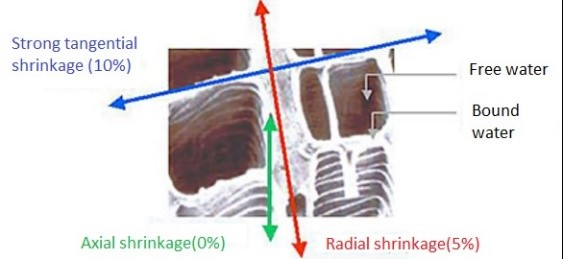
\includegraphics[width=8cm]{fig6}
	\caption{3 types of wood shrinkage}
	\label{fig:galaxy}
\end{figure}

\subsection{Influence of density on wood}

Density is the ratio of the density of wood to that of water. Wood can change in weight and volume as a result of moisture gain and loss. Generally the reference density is calculated with 12\% moisture. In fact, some researchers have shown that Young's modulus, Poisson's ratio and shear modulus depend on wood density[HEI 2013]. The density of wood varies from one species to another and also within the same species. The more fibers the wood has, the denser it is. If we take the example of balsa, it has a low proportion of fibers and therefore a low density. Conversely, panacoco has a high proportion of fibers and therefore has a high density[THI 2015].

Bodig and Jayne [BOD 1982]  developed a formula that relates the mechanical properties of the generalized Hooke's law to the density of wood by the relation :

\begin{equation}
	Y = a*D^b
\end{equation}

where Y represents the elastic properties, D is the density of the wood, a and b are two constants given in the charts for each wood species.

The density is expressed by the following formula:

\begin{equation}
	\rho = \frac{\rho_{woodspecimen}}{\rho_{4degreewater}}
\end{equation}

\subsection{Mechanical properties}

From a mechanical point of view, wood is an anisotropic material (= physical and mechanical properties depending on the direction considered) and orthotropic (it has 3 preferred directions: axial, radial, tangential). 

Wood is considered as an elastic material. It means that wood will return to its original shape or dimensions when the load causing the deformation is removed. Beyond this load limit, the wood does not regain its shape. It has then reached the plastic domain. It is the presence of cellulose that gives the wood a linear elastic behaviour. By drawing the stress-strain curve, it is possible to determine the Young's modulus E.

\graphicspath{{Images/}}
\begin{figure}[htp]
	\centering
	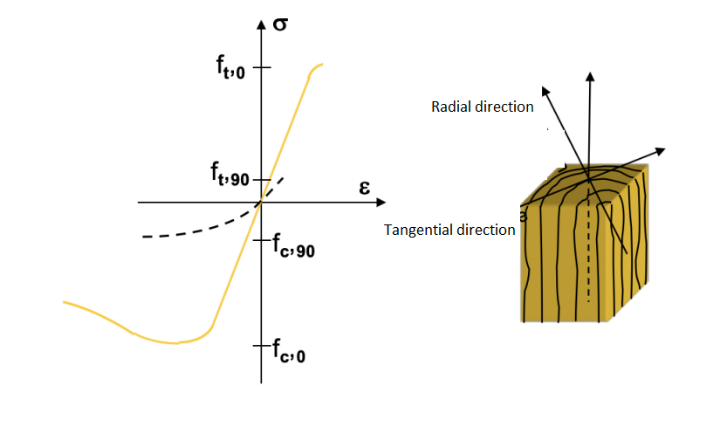
\includegraphics[width=8cm]{fig7}
	\caption{Orthotropy of wood without defects [TAA 2022]}
	\label{fig:galaxy}
\end{figure}

The curves in Figure 6 show the compressive and tensile behaviour of flawless wood loaded parallel to the fibres (solid line) and perpendicularly (dashed line) at a constant strain rate. Cellulose provides high mechanical properties in the longitudinal direction, as this is the direction in which it is oriented. In the transverse direction, the little cohesion provided by the lignin is not sufficient to hold the fibres together, only the radial tracheids provide a little strength. It can be said that wood without defects has a strong anisotropy. It is rigid and strong parallel to the fibres, sensitive to splitting and has low shear strength [TAA 2022].

Considering a one-dimensional behavior model in the direction of the fibers, we can write :

\begin{equation}
	\sigma = E_{L}*\epsilon
\end{equation}

With the proportionality between the stress $\sigma$ and the deformation $\epsilon$ along the fiber axis with respect to the wood grain, $ E_L $ represents the "longitudinal modulus of elasticity" which must in all rigor be characterized for each load case in tension, compression, bending etc.

\newpage

\textbf{Compression wood}

In order to determine the behaviour of the material in compression, it must be stressed in both directions (parallel and orthogonal to the fibres). This is known as axial compression and transverse compression. The test is carried out on a parallelepipedic specimen, 20 x 20 x 60  with a loading speed of 40 MPa/mm. The variation of the stress as a function of the strain is plotted on the figure 6:

\graphicspath{{Images/}}
\begin{figure}[htp]
	\centering
	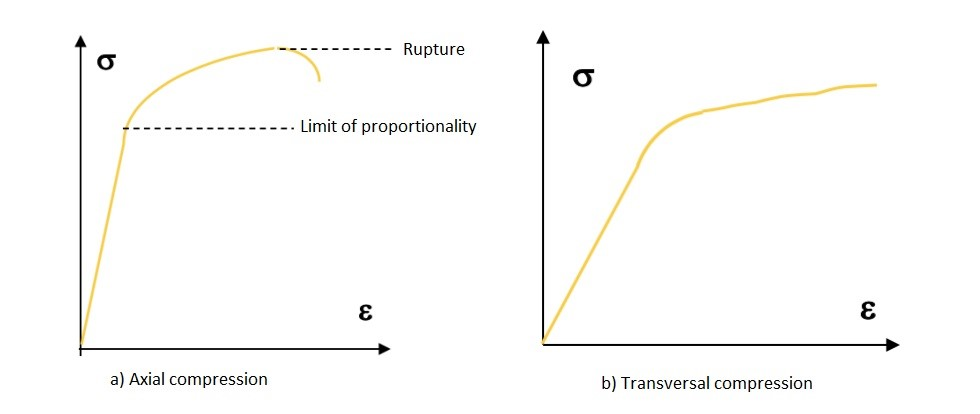
\includegraphics[width=8cm]{fig8}
	\caption{Axial and transverse compression of wood}
	\label{fig:galaxy}
\end{figure}

Orders of magnitude of axial compressive strengths and elastic moduli can be given for each type of wood species in table 2: 

\graphicspath{{Images/}}
\begin{figure}[htp]
	\centering
	
\includegraphics[width=8cm]{fig9}
	\caption{Orders of magnitude of axial compressive strengths and elastic moduli}
	\label{fig:galaxy}
\end{figure}

For transverse compression and regardless of the wood species, the strength is divided by 7 (i.e. strength < 10 MPa). 

The strength of the wood can then be assessed if it is loaded obliquely, i.e. the direction of loading is at an angle of 0 to 90° to the direction of the fibres (angle a). 

\graphicspath{{Images/}}
\begin{figure}[htp]
	\centering
	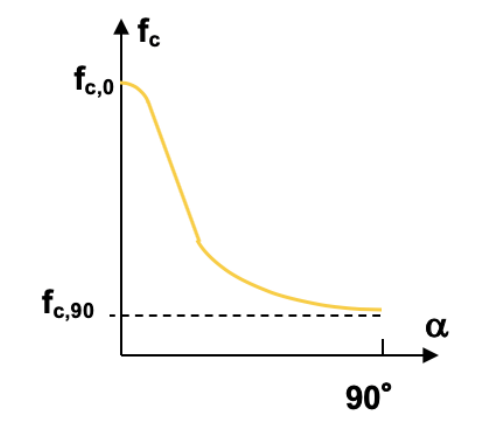
\includegraphics[width=8cm]{fig10}
	\caption{Variation of the compressive strength of wood as a function of the load angle}
	\label{fig:galaxy}
\end{figure}

Figure 7 shows the variation of the compressive strength of wood as a function of the load angle. It can be seen that the strength is maximum for a load parallel to the fibres (fc,0) and minimum for a load perpendicular to the fibres (fc,90). Theoretically, the compressive strength can be evaluated as a function of this angle a using the Hankinson formula equation 1. A similar formula exists for the modulus.

\begin{equation}
	\sigma_{\alpha} = \frac{\sigma_{0}*\sigma_{90}}{\sigma_{\alpha}*sin(\alpha)^2+\sigma_{90}*cos(\alpha)^2}
\end{equation}

Wood has an almost elastic tensile behaviour until it breaks. Its tensile elastic modulus is equivalent to that in axial compression. The breaking stress is up to twice as high as that in compression. We can retain $f_{t0}=80$ to 140 MPa.

\graphicspath{{Images/}}
\begin{figure}[htp]
	\centering
	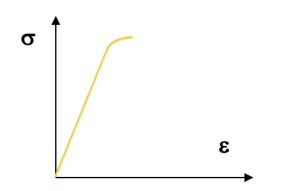
\includegraphics[width=8cm]{fig11}
	\caption{Variation of the axial tensile stress of wood with deformation}
	\label{fig:galaxy}
\end{figure}

In the same way as for compression, the oblique tensile strength can be theoretically evaluated using the Hankinson formula. However, these values are strongly influenced by the presence of knots and the possible slope of the wood grain.

\smallskip

\textbf{Wood shearing}

In order to measure the shear strength of wood in the longitudinal direction, a preferential shear plane must be created by the shape of the specimen. This is illustrated in Figure 8 :

\graphicspath{{Images/}}
\begin{figure}[htp]
	\centering
	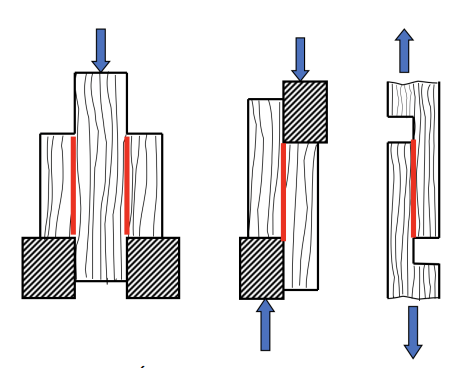
\includegraphics[width=8cm]{fig12}
	\caption{Wood shearing}
	\label{fig:galaxy}
\end{figure}

In the figure, the light areas represent the wood, the dark areas represent the blocking points (prevented displacement) and the arrows represent the stresses. These experimental set-ups allow the creation of shear planes (in red). These shear strength values can be retained in table 3 :

\graphicspath{{Images/}}
\begin{figure}[htp]
	\centering
	
\includegraphics[width=10cm]{fig13}
	\caption{Shear strenght values}
	\label{fig:galaxy}
\end{figure}

\section{Conclusion}

This chapter will have provided a better understanding of the material wood. Its definition, its various functions, its physical and mechanical properties were reminded as well as the elements which constitute it at the macroscopic and microscopic level. Moreover, it was also recalled the various parameters such as moisture that can influence the physical and mechanical characteristics of wood.
The following chapter will present the fracture mechanics tools for the study of cracking and the experimental measurement technique used.


